\documentclass[12pt]{article}
\usepackage{graphicx}

\begin{document}
\textbf{\huge{Signal System and Control}}

\begin{center}
\large{Laboratory 1}
\end{center}

\begin{flushright}
Piotr Czajka

251677
\end{flushright}

\section{Exercises}

\subsection{Exercise 1}

Relationship between the Levinson algorithm convergence speed and the bandwidth of the parametrized signal.

\vspace{1cm}

We are interested in following charts:

Fist signal frequency is: 0.1

Second signal frequency is: 0.2

Bandwith is: 0.1

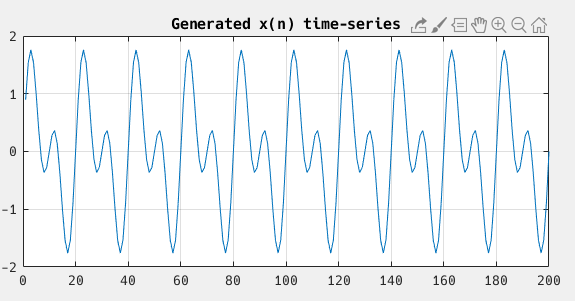
\includegraphics[width=\textwidth]{1.png}

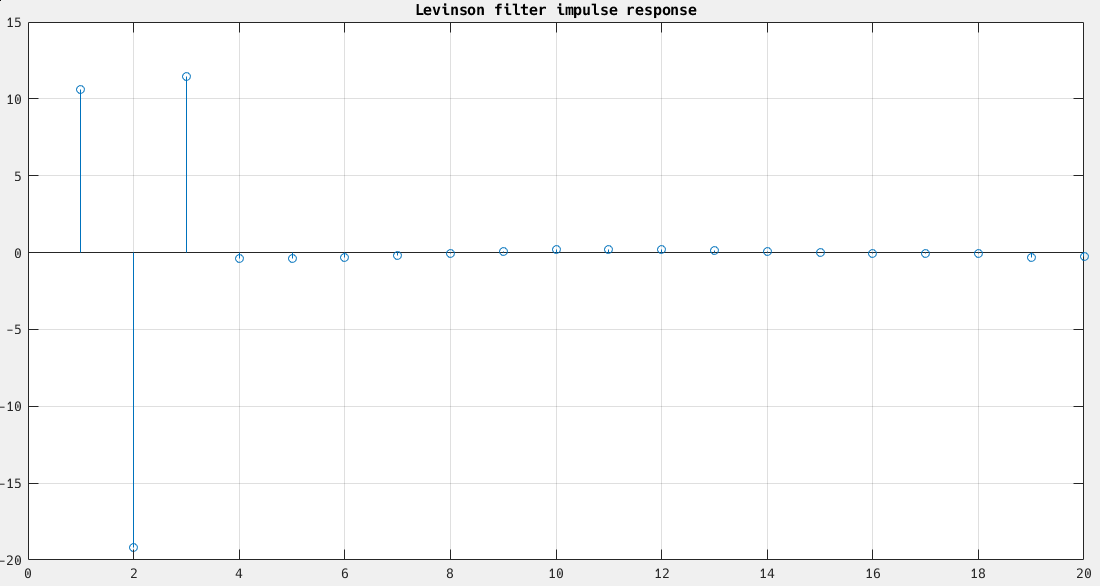
\includegraphics[width=\textwidth]{2.png}

\vspace{1cm}

First signal frequency: 0.1

Second signal frequency: 0.5

Third signal frequency: 0.9

Bandwidth is 0.8

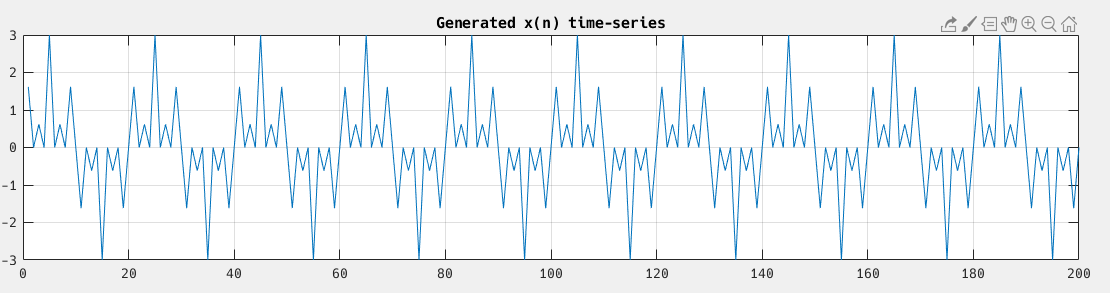
\includegraphics[width=\textwidth]{3.png}

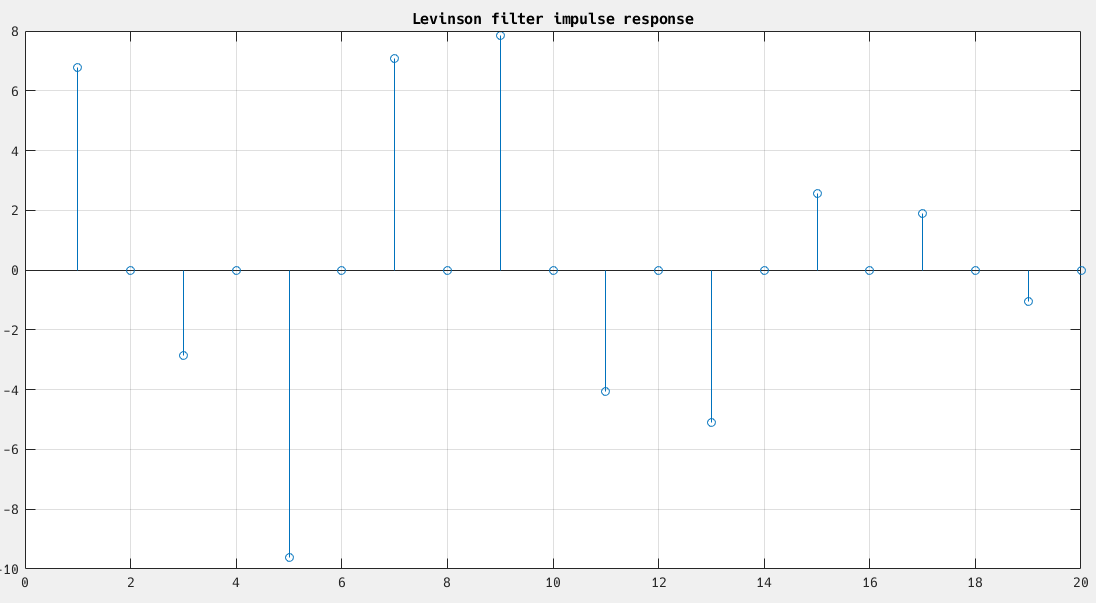
\includegraphics[width=\textwidth]{4.png}

When we increase the bandwidth, it slows down the convergende speed.

\subsection{Exercise 2}

How does placement of the PSD signal and bandwidth affects convergence speed?

Looking at following charts:

First freq: 0.1

Second freq: 0.2

Bandwidth: 0.1

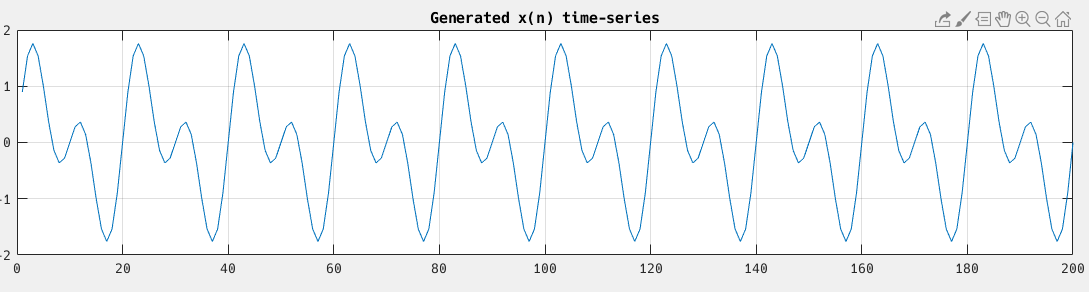
\includegraphics[width=\textwidth]{5.png}

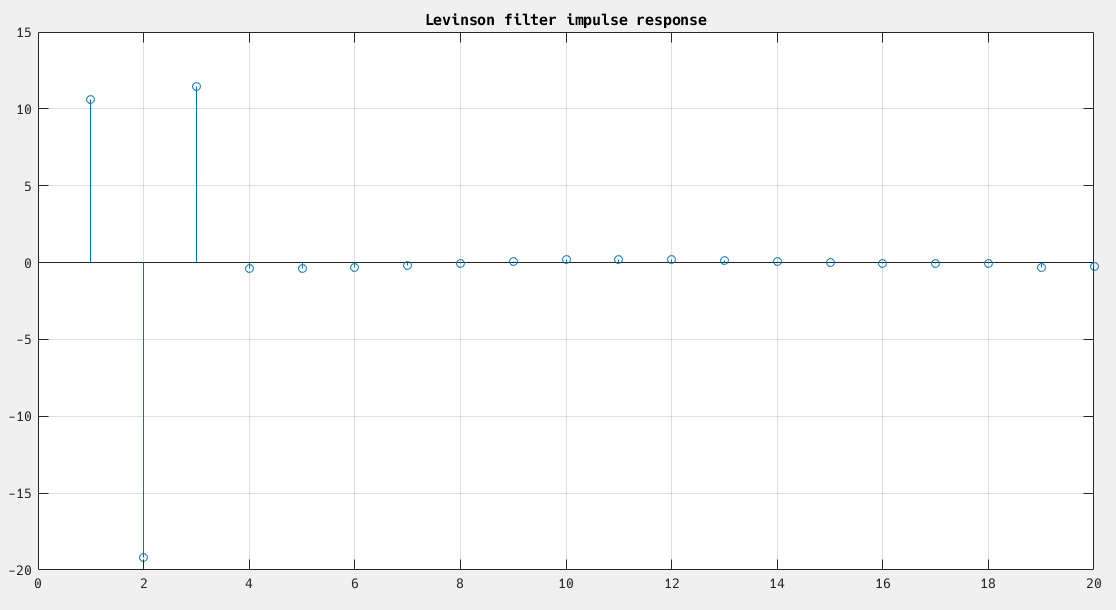
\includegraphics[width=\textwidth]{6.png}

First freq: 0.7

Second freq: 0.8

Bandwidth: 0.1

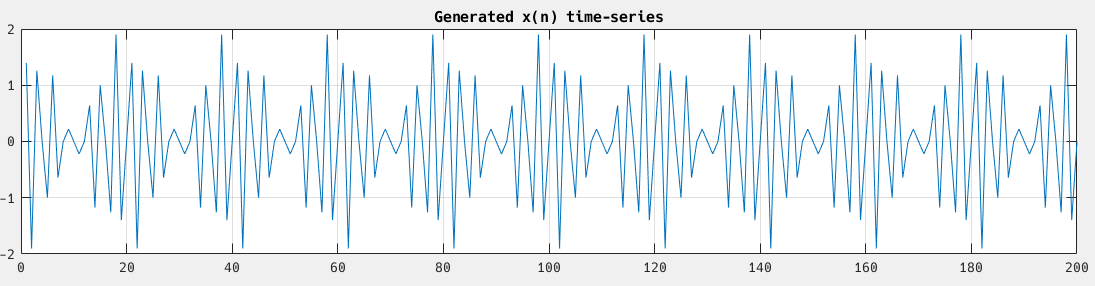
\includegraphics[width=\textwidth]{7.png}

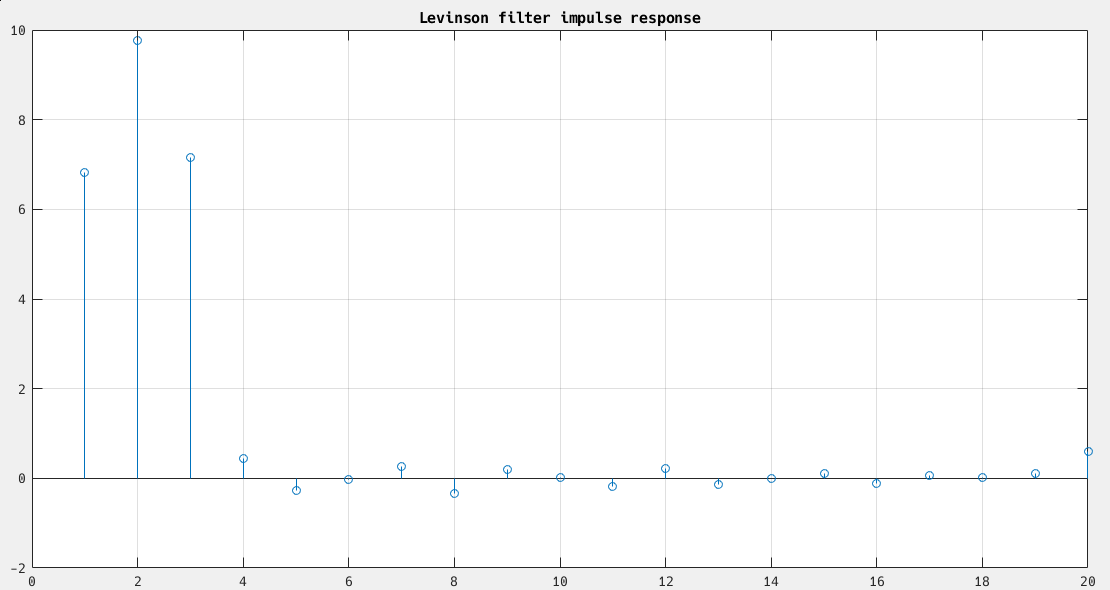
\includegraphics[width=\textwidth]{8.png}

First freq: 0.4

Second freq: 0.8

Bandwidth: 0.4

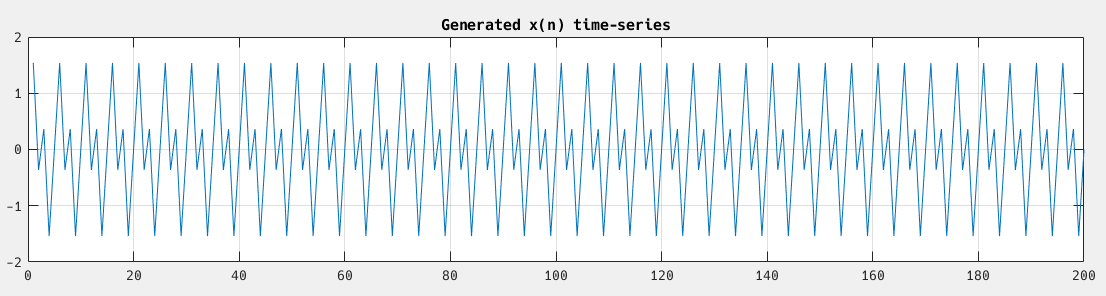
\includegraphics[width=\textwidth]{9.png}

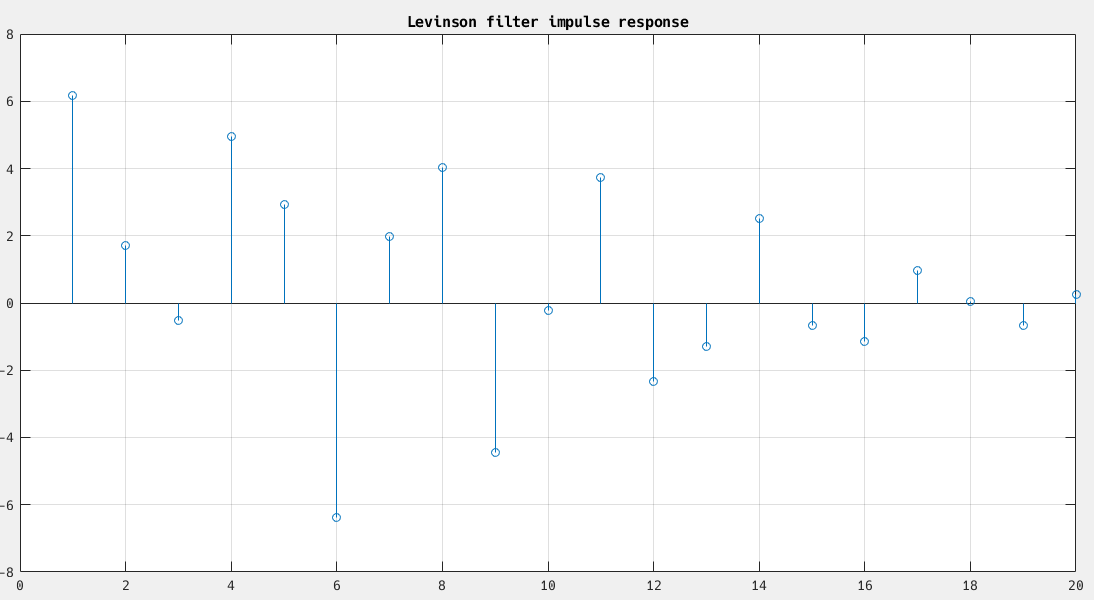
\includegraphics[width=\textwidth]{10.png}

We could conclude, that signal offset does not affect the convergence speed. The bandwidth does.

\subsection{Exercise 3}

Correlation between Shur coefficient values and the number of signal components

We can see this on the following charts:

For one sinusoid signal:

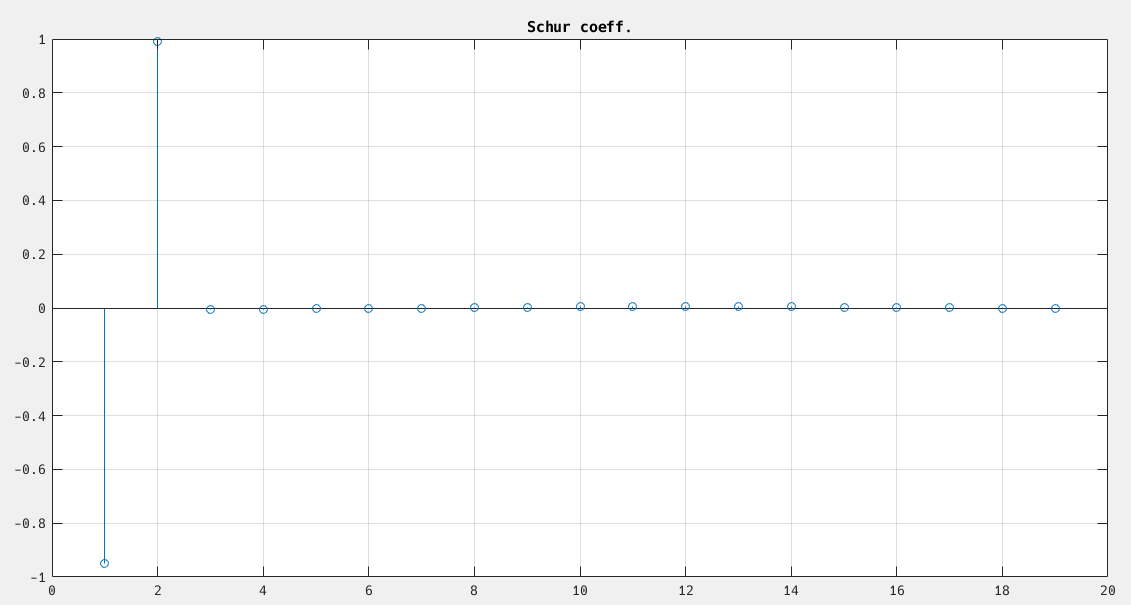
\includegraphics[width=\textwidth]{11.png}

Two sinusoids:

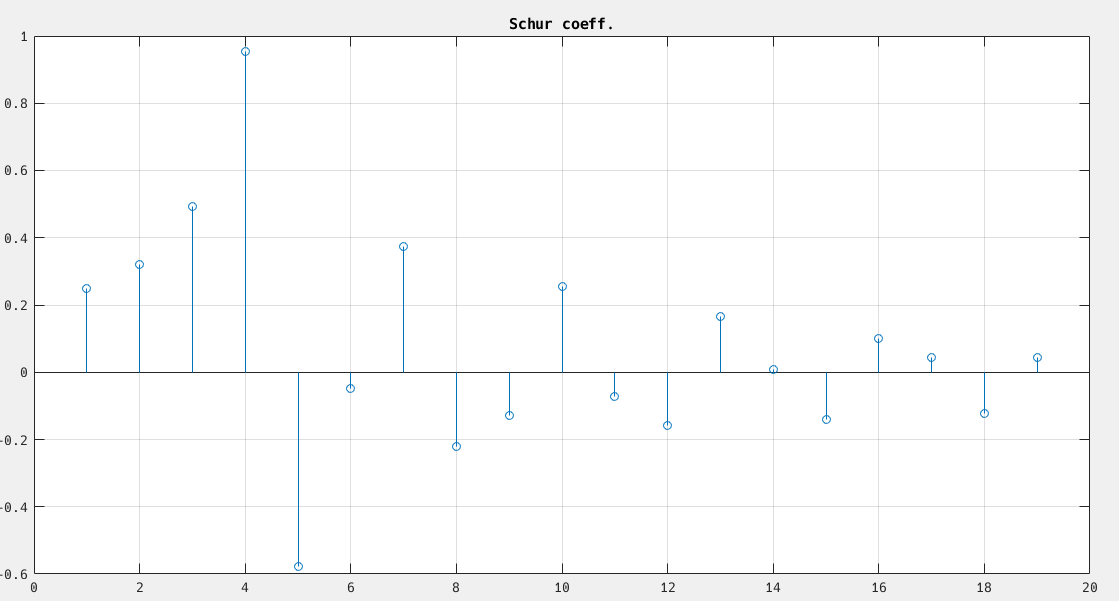
\includegraphics[width=\textwidth]{12.png}

Three sinusoids:

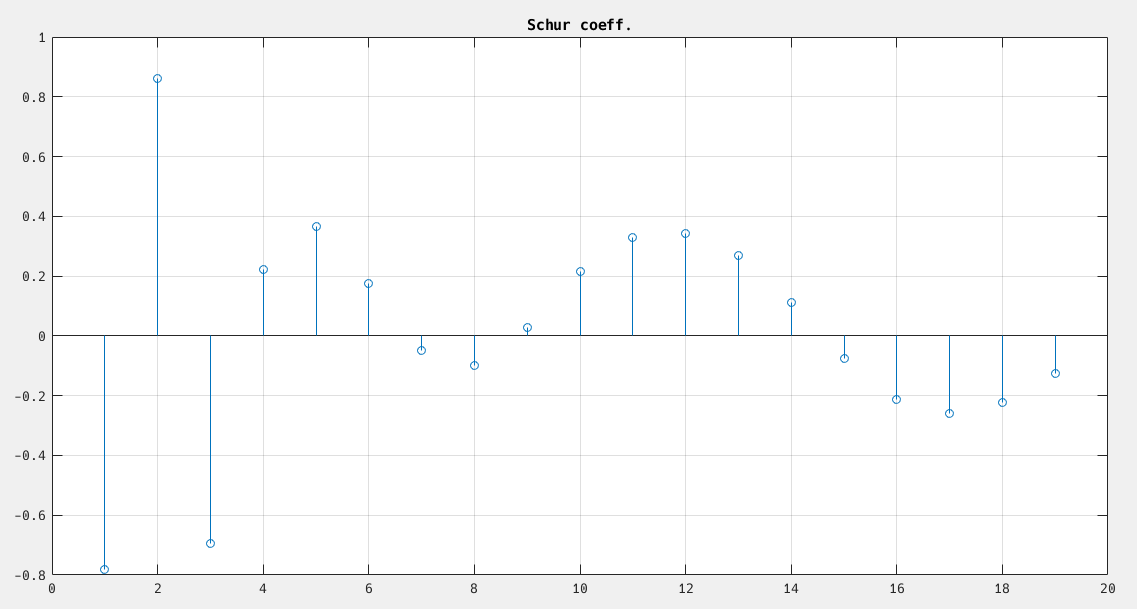
\includegraphics[width=\textwidth]{13.png}

The more signal is complicated the more non-zero Schur values it has.

\subsection{Exercise 4}

Relation with magniture Levinson filter characteristic and PSD of the input.

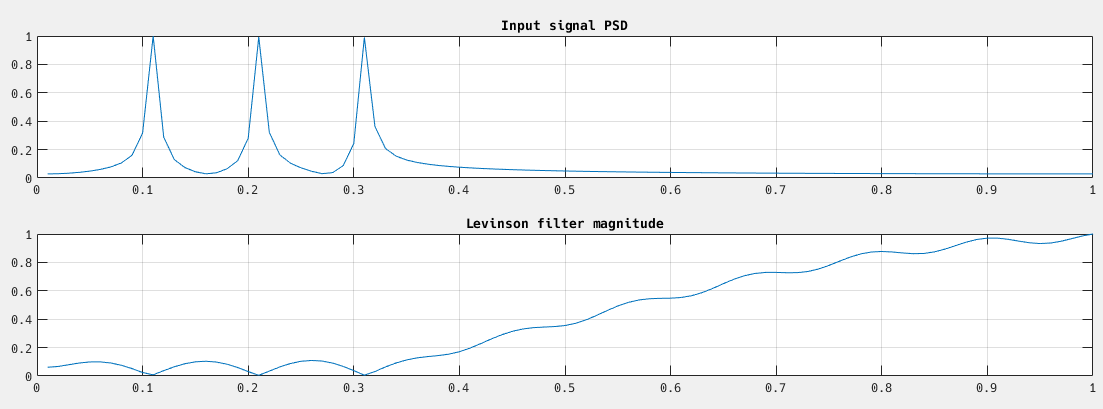
\includegraphics[width=\textwidth]{14.png}

We can see, that when the input signal PSD reaches it maximums, Levinson fileter magnitude reaches it's minumums.

\subsection{Exercise 5}

Comparasion with real life signals

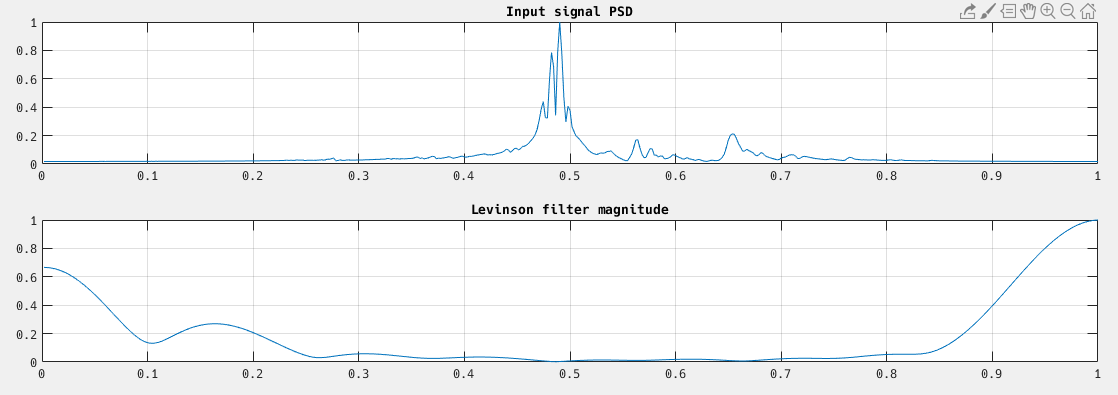
\includegraphics[width=\textwidth]{15.png}

In here, when input signal PSD reaches it's maximum, Levinson magnitude is in the minumum.

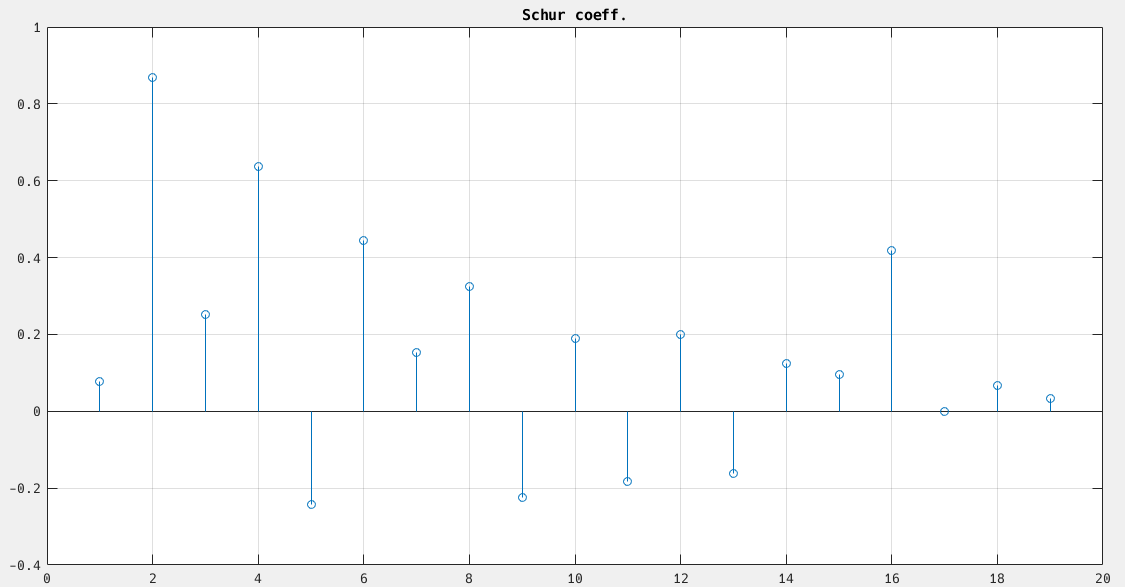
\includegraphics[width=\textwidth]{16.png}

Signal is very complicated, so there are many non-zero Schur values.

\end{document}
